\chapter{Contexte Général}

\section{Introduction}

Ce chapitre établit le contexte dans lequel VM Marketplace a été conçue et développée.
Nous présentons d'abord l'organisme d'accueil, puis nous situons le projet dans le
paysage cloud académique tunisien, définissons la problématique, étudions les solutions
existantes, proposons notre réponse et justifions la méthodologie de développement
adoptée.

% ─────────────────────────────────────────────────────────────────────────────
\section{Présentation de l'Organisme d'Accueil}
% ─────────────────────────────────────────────────────────────────────────────

\subsection{Informations Générales}

Huawei Technologies Co., Ltd.\ est une multinationale chinoise de technologie fondée
en 1987 à Shenzhen, Chine, par Ren Zhengfei. Elle est aujourd'hui l'un des plus grands
fournisseurs mondiaux d'infrastructure TIC (Technologies de l'Information et de la
Communication) et de dispositifs intelligents, avec des activités dans plus de
170 pays et un chiffre d'affaires dépassant 92 milliards de dollars en
2023~\cite{huawei2023annual}.

\textbf{Huawei Technologies Tunisie} est la filiale locale chargée du déploiement
des solutions entreprise et gouvernementales de Huawei sur le marché nord-africain.
En Tunisie, la société a établi un partenariat stratégique avec le MESRS pour fournir
et opérer l'infrastructure nationale \textbf{Huawei Cloud Stack (HCS)} au profit des
institutions académiques~\cite{mesrs_hcs}.

\subsection{Huawei Cloud Stack (HCS)}

Huawei Cloud Stack est la plateforme cloud on-premises de Huawei, conçue pour les
déploiements gouvernementaux et d'entreprise où la souveraineté des données exige que
les ressources de calcul restent dans un périmètre physique contrôlé. Le déploiement
MESRS, accessible à l'adresse \textit{mesrscloud.rnu.tn}, met à disposition des
universités et laboratoires de recherche des instances ECS (Elastic Cloud Server), des
réseaux VPC (Virtual Private Cloud), des adresses IP élastiques (EIP) et du stockage
objet~\cite{hcs_docs}.

HCS expose des API compatibles OpenStack, et Huawei distribue un fournisseur Terraform
officiel (\texttt{huaweicloud/hcs}) permettant la gestion en infrastructure as code
de toutes les ressources cloud~\cite{hcs_terraform_provider}.

\subsection{Contexte du Stage}

Le stage s'est déroulé au sein de l'équipe Infrastructure Cloud de Huawei Technologies
Tunisie. L'équipe est responsable de la maintenance du déploiement HCS et de
l'assistance technique aux institutions académiques. La mission de la stagiaire
consistait à concevoir et livrer un portail en libre-service réduisant la charge
manuelle des administrateurs tout en donnant de l'autonomie aux utilisateurs finaux.

% ─────────────────────────────────────────────────────────────────────────────
\section{Contexte du Projet et Problématique}
% ─────────────────────────────────────────────────────────────────────────────

\subsection{Contexte du Projet}

Les chercheurs et étudiants des universités tunisiennes ont fréquemment besoin de
machines virtuelles pour leurs expériences computationnelles, analyses de données et
charges de travail containerisées. L'accès à la plateforme HCS MESRS nécessite
actuellement de soumettre une demande à un administrateur, qui provisionne
manuellement la ressource et communique les identifiants par e-mail. Ce processus
introduit des délais de plusieurs jours à plusieurs semaines, ne laisse aucune
autonomie à l'utilisateur, ne génère aucune traçabilité et laisse la supervision
entièrement à la charge de l'utilisateur une fois l'accès accordé.

Par ailleurs, les utilisateurs non experts --- tels que les étudiants novices en
cloud computing --- n'ont aucun guide pour choisir la configuration de VM adaptée
à leur charge de travail, ce qui crée un risque de sur-provisionnement (gaspillage de
quota) ou de sous-provisionnement (performances dégradées).

\subsection{Problématique}

La problématique adressée par ce projet peut être formulée comme suit :

\begin{quote}
\textit{« Comment une plateforme web en libre-service peut-elle permettre aux
utilisateurs académiques du cloud HCS MESRS de provisionner et gérer de façon
autonome des machines virtuelles et des clusters Kubernetes, avec intégration du
paiement, recommandation IA de configuration, suivi en temps réel du provisionnement
et supervision automatisée --- tout en opérant dans les contraintes de quota de
ressources de l'environnement HCS partagé ? »}
\end{quote}

% ─────────────────────────────────────────────────────────────────────────────
\section{Étude de l'Existant}
% ─────────────────────────────────────────────────────────────────────────────

\subsection{Présentation des Solutions Candidates}

Plusieurs plateformes existantes abordent la problématique du libre-service cloud.
Nous avons étudié quatre solutions représentatives pour identifier leurs capacités
et leurs limites dans le contexte de l'environnement HCS MESRS.

\paragraph{OpenStack Horizon.}
Horizon est le tableau de bord web officiel d'OpenStack~\cite{horizon_docs}.
Il offre une interface de libre-service complète pour lancer des instances, gérer des
réseaux et configurer des groupes de sécurité. HCS étant compatible OpenStack, Horizon
pourrait théoriquement être déployé face aux API MESRS.

\paragraph{Proxmox VE.}
Proxmox Virtual Environment est une plateforme open source de gestion d'hyperviseur
qui propose une interface web intégrée pour la gestion du cycle de vie des VM et
conteneurs~\cite{proxmox_docs}. Elle est largement utilisée dans les établissements
d'enseignement pour les environnements de laboratoire.

\paragraph{VMware Cloud Director.}
VMware Cloud Director propose un portail cloud multi-tenant pour l'infrastructure
vSphere~\cite{vmware_vcd}. Il offre des capacités de libre-service étendues incluant
les modèles de VM, la configuration réseau et la facturation.

\paragraph{AWS Management Console.}
La console de gestion AWS est la référence de facto des portails de libre-service
cloud~\cite{aws_console}. Elle propose une interface riche et intuitive pour tous
les services AWS incluant EC2, EKS et IAM.

\subsection{Analyse Comparative}

Le tableau~\ref{tab:existing_solutions} résume les capacités clés de chaque solution
face aux exigences du contexte MESRS.

\begin{table}[H]
\centering
\caption{Comparaison des solutions cloud en libre-service existantes}
\label{tab:existing_solutions}
\begin{tabularx}{\linewidth}{lXXXXX}
\toprule
\textbf{Critère}         & \textbf{OpenStack Horizon} & \textbf{Proxmox VE}
                         & \textbf{VMware VCD}        & \textbf{AWS Console}
                         & \textbf{VM Marketplace (proposé)} \\
\midrule
Compatibilité HCS        & Partielle & \xmark & \xmark & \xmark & \cmark \\
Intégration paiement     & \xmark    & \xmark & \cmark & \cmark & \cmark \\
Recommandation IA        & \xmark    & \xmark & \xmark & \xmark & \cmark \\
Suivi SSE temps réel     & \xmark    & \xmark & \xmark & Partiel & \cmark \\
Terminal SSH navigateur  & \xmark    & \cmark & \xmark & \xmark & \cmark \\
Supervision automatisée  & \xmark    & Partiel & Partiel & Partiel & \cmark \\
Provisionnement K8s      & Partiel   & \xmark & Partiel & \cmark & \cmark \\
LLM local (sans API cloud)& \xmark   & \xmark & \xmark & \xmark & \cmark \\
Open source / gratuit    & \cmark    & \cmark & \xmark & \xmark & \cmark \\
\bottomrule
\end{tabularx}
\end{table}

% ─────────────────────────────────────────────────────────────────────────────
\section{Critique de l'Existant}
% ─────────────────────────────────────────────────────────────────────────────

L'étude révèle les limites suivantes des plateformes existantes dans le contexte MESRS :

\begin{itemize}
  \item \textbf{Absence d'intégration HCS native.} Aucune plateforme commerciale ne
        supporte le fournisseur Terraform \texttt{huaweicloud/hcs} ni les endpoints
        d'API spécifiques à HCS (type EIP \texttt{External-01}, résolution de flavor
        par nom).

  \item \textbf{Absence de guide IA.} Toutes les solutions existantes supposent que
        les utilisateurs connaissent déjà le type d'instance adapté à leur charge de
        travail. Les utilisateurs non experts ne bénéficient d'aucune assistance
        dans la plateforme.

  \item \textbf{Absence d'intégration du paiement.} À l'exception des offres
        commerciales (VMware VCD, AWS), aucune solution n'intègre de flux de paiement,
        pourtant nécessaires pour un modèle de crédit académique à l'usage.

  \item \textbf{Absence de suivi SSE en temps réel.} Les portails existants ne
        diffusent pas la progression étape par étape du provisionnement vers le
        navigateur, laissant les utilisateurs dans l'incertitude lors des opérations
        longues.

  \item \textbf{Absence d'intégration de supervision.} Les utilisateurs doivent
        installer leurs propres outils de monitoring après la création de la VM, ce
        qui requiert une expertise d'administration cloud que beaucoup d'utilisateurs
        académiques ne possèdent pas.

  \item \textbf{Confidentialité pour l'IA.} AWS, Azure et GCP proposent une
        assistance IA pour la sélection de ressources, mais ils envoient les
        descriptions de charge de travail des utilisateurs à des API cloud externes.
        Dans un contexte de recherche avec des données sensibles, un LLM hébergé
        localement est fortement préférable.
\end{itemize}

% ─────────────────────────────────────────────────────────────────────────────
\section{Solution Proposée}
% ─────────────────────────────────────────────────────────────────────────────

\subsection{Vue d'Ensemble}

VM Marketplace est une plateforme de gestion cloud en libre-service conçue
spécifiquement pour l'environnement HCS MESRS. Elle permet aux utilisateurs
authentifiés de configurer, payer, provisionner, accéder et superviser des machines
virtuelles et des clusters Kubernetes entièrement via un navigateur, sans aucune
intervention d'un administrateur.

La plateforme se différencie des solutions existantes sur quatre axes :
\begin{enumerate}
  \item \textbf{Native HCS :} toutes les opérations de provisionnement utilisent le
        fournisseur Terraform officiel \texttt{huaweicloud/hcs}, garantissant une
        compatibilité totale avec l'environnement de production MESRS.
  \item \textbf{Assistée par IA :} un LLM Llama~3.1 hébergé localement traduit des
        descriptions textuelles de charge de travail en recommandations concrètes de
        flavor HCS, rendant la plateforme accessible aux non-experts.
  \item \textbf{Transparente :} des Server-Sent Events en temps réel diffusent chaque
        étape du provisionnement vers le navigateur de l'utilisateur, éliminant
        l'incertitude durant les 5 à 10 minutes d'exécution Terraform.
  \item \textbf{Cycle de vie intégré :} du paiement à l'accès SSH en passant par les
        tableaux de bord de supervision et le téléchargement du kubeconfig, l'ensemble
        du cycle de vie est géré au sein d'une seule plateforme.
\end{enumerate}

\subsection{Architecture Générale}

La plateforme se compose de trois services indépendants, comme illustré dans la
figure~\ref{fig:highlevel_arch}.

\begin{figure}[H]
  \centering
  \begin{tikzpicture}[
    node distance=1.5cm and 2.5cm,
    box/.style={rectangle, draw, rounded corners=4pt, minimum width=3.5cm,
                minimum height=1.2cm, align=center, font=\small\bfseries},
    cloud/.style={ellipse, draw, minimum width=3cm, minimum height=1.2cm,
                  align=center, font=\small\bfseries, fill=blue!10},
    arr/.style={-{Stealth}, thick},
  ]
    \node[box, fill=green!10]  (fe)  {Frontend Next.js\\(port 3000)};
    \node[box, fill=orange!10] (be)  [right=of fe] {Backend FastAPI\\(port 8000)};
    \node[box, fill=purple!10] (ai)  [below=of be] {Moteur IA\\(port 8001)};
    \node[cloud, fill=blue!10] (hcs) [right=of be] {Cloud HCS\\mesrscloud.rnu.tn};
    \node[box, fill=gray!10]   (tf)  [below=of hcs] {Terraform\\huaweicloud/hcs};

    \draw[arr] (fe) -- node[above,font=\scriptsize]{REST / SSE / WS} (be);
    \draw[arr] (be) -- node[left,font=\scriptsize]{/api/ai/recommend} (ai);
    \draw[arr] (be) -- node[above,font=\scriptsize]{Appels API} (hcs);
    \draw[arr] (be) -- node[right,font=\scriptsize]{sous-processus} (tf);
    \draw[arr] (tf) -- (hcs);
  \end{tikzpicture}
  \caption{Architecture générale de VM Marketplace}
  \label{fig:highlevel_arch}
\end{figure}

% ─────────────────────────────────────────────────────────────────────────────
\section{Méthodologie}
% ─────────────────────────────────────────────────────────────────────────────

\subsection{Comparaison des Méthodologies de Développement}

Le tableau~\ref{tab:methodologies} compare trois méthodologies candidates face aux
contraintes de ce projet : un développeur unique, une durée de six mois, des
contraintes d'environnement HCS évolutives et une livraison de fonctionnalités
incrémentale.

\begin{table}[H]
\centering
\caption{Comparaison des méthodologies de développement}
\label{tab:methodologies}
\begin{tabularx}{\linewidth}{lXXX}
\toprule
\textbf{Critère}               & \textbf{Cascade} & \textbf{Modèle en V} & \textbf{Agile/Scrum} \\
\midrule
Adaptabilité au changement     & Faible   & Faible   & Élevée \\
Livraison de valeur précoce    & Faible   & Faible   & Élevée \\
Adapté au développeur solo     & Oui      & Oui      & Oui \\
Gestion des inconnues externes & Faible   & Faible   & Élevée \\
Charge documentaire            & Élevée   & Élevée   & Modérée \\
Validation intégrée            & En fin   & Parallèle & À chaque sprint \\
\bottomrule
\end{tabularx}
\end{table}

\subsection{Méthodologie Retenue : Agile Itératif}

Compte tenu des nombreuses contraintes imprévues de l'environnement HCS (limitations
de quota, politiques d'authentification SSH, règles de transfert réseau au niveau de
l'hyperviseur), une approche de planification rigide aurait été inadaptée. Nous avons
adopté une approche \textbf{Agile itérative} organisée en trois sprints, chacun livrant
une tranche verticale fonctionnelle de la plateforme :

\begin{itemize}
  \item \textbf{Sprint 1 :} Authentification utilisateur, assistant de configuration
        de VM, provisionnement Terraform, intégration du paiement Stripe.
  \item \textbf{Sprint 2 :} Moteur de recommandation IA, terminal SSH dans le
        navigateur, installation de la supervision Netdata.
  \item \textbf{Sprint 3 :} Provisionnement de clusters Kubernetes avec solution
        réseau complète pour les nœuds workers privés.
\end{itemize}

Chaque sprint a livré un ensemble de fonctionnalités démontrable et testable. Les
problèmes découverts dans l'environnement HCS (épuisement du quota EIP, politique SSH
à clé publique uniquement, \texttt{source\_dest\_check} au niveau de l'hyperviseur)
ont été traités au sein du sprint par itération rapide.

\subsection{Planification du Projet}

La figure~\ref{fig:gantt} présente le diagramme de Gantt du projet sur six mois.

\begin{figure}[H]
\centering
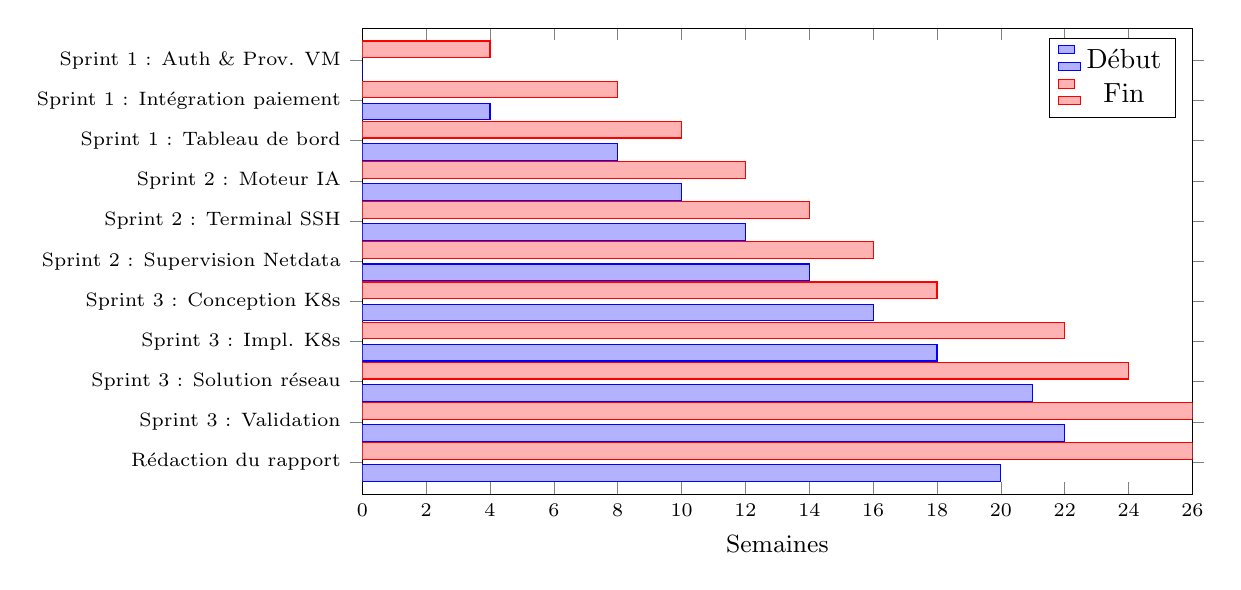
\begin{tikzpicture}
  \begin{axis}[
    xbar,
    y dir=reverse,
    xlabel={Semaines},
    ytick=data,
    yticklabels={
      {Sprint 1 : Auth \& Prov. VM},
      {Sprint 1 : Intégration paiement},
      {Sprint 1 : Tableau de bord},
      {Sprint 2 : Moteur IA},
      {Sprint 2 : Terminal SSH},
      {Sprint 2 : Supervision Netdata},
      {Sprint 3 : Conception K8s},
      {Sprint 3 : Impl. K8s},
      {Sprint 3 : Solution réseau},
      {Sprint 3 : Validation},
      {Rédaction du rapport}
    },
    xmin=0, xmax=26,
    bar width=6pt,
    width=\linewidth,
    height=7.5cm,
    enlarge y limits=0.08,
    tick label style={font=\scriptsize},
    label style={font=\small},
  ]
  \addplot coordinates {
    (0,0) (4,1) (8,2) (10,3) (12,4) (14,5) (16,6) (18,7) (21,8) (22,9) (20,10)
  };
  \addplot coordinates {
    (4,0) (8,1) (10,2) (12,3) (14,4) (16,5) (18,6) (22,7) (24,8) (26,9) (26,10)
  };
  \legend{Début, Fin}
  \end{axis}
\end{tikzpicture}
\caption{Diagramme de Gantt --- planification du projet VM Marketplace
([TODO : ajuster les numéros de semaines selon la date de début réelle du stage])}
\label{fig:gantt}
\end{figure}

% ─────────────────────────────────────────────────────────────────────────────
\section{Conclusion}
% ─────────────────────────────────────────────────────────────────────────────

Ce chapitre a situé VM Marketplace dans l'écosystème cloud académique du MESRS,
identifié les lacunes des solutions existantes et défini le périmètre de la plateforme
proposée. La méthodologie Agile itérative, organisée en trois sprints ciblés, a été
choisie pour gérer les contraintes imprévisibles de l'environnement HCS de production.
Le chapitre suivant formalise les besoins fonctionnels et non fonctionnels, et
établit l'architecture technique de la solution.
